

\section{Sampling}


\begin{frame}
\Huge{\centerline{Part 2}}
\end{frame}

\begin{frame}
\frametitle{Sampling \& Concentration Inequalities}

\begin{block}{Research Question}
How can we select samples in Stratified Sampling \& Shapley Value Approximation better?
\end{block}

Orthodox answer, is that you select samples in proportion to the size \& variance of the strata.
\begin{theorem}[Neyman allocation]\label{thm:neyman_selection}
For strata of sizes $N_i$, with variance $\sigma_i^2$ for a sample budget $n$ the $n_i$ which minimises the variance of our population estimate $\mu$ is:
$$n_i = n\frac{N_i\sigma_i}{\sum_jN_j\sigma_j}$$
\end{theorem}
\end{frame}


\begin{frame}
\begin{figure}
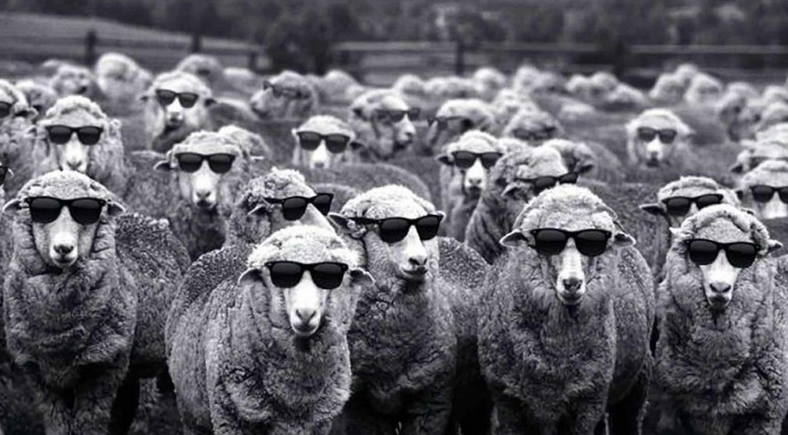
\includegraphics[width=0.45\linewidth,height=0.25\linewidth]{figs/sheep.png}%
$~~~~~$
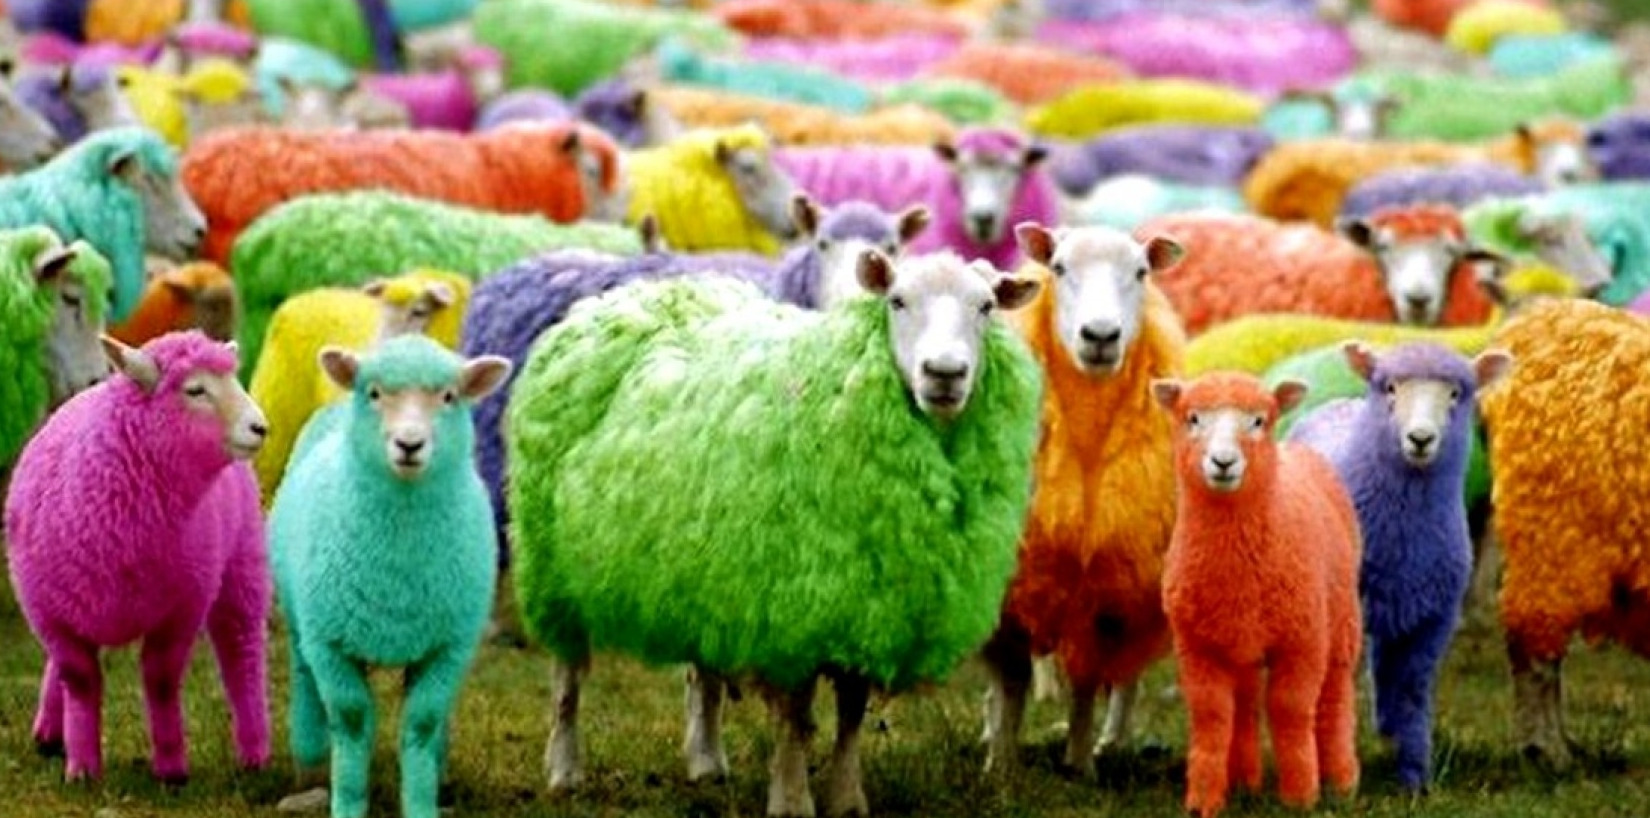
\includegraphics[width=0.45\linewidth,height=0.25\linewidth]{figs/sheep2.jpg}%
\end{figure}
Sampling in proportion to strata variance$\times$size is intuitive, extends from Chebyshev's inequality:
\begin{theorem}[Chebyshev's inequality]\label{thm:chebyshevs}
for any random variable $\hat{\mu}$ with variance $\text{Var}(\hat{\mu})$ then the error of $\hat{\mu}$ from its mean is probability bounded:
$$ \p\left(|\hat{\mu}-\mu|\ge k\sqrt{\text{Var}(\hat{\mu})}\right)\le\frac{1}{k^2} $$
\end{theorem}
Problem is... that we dont know the variances in practice.
\end{frame}


\begin{frame}
\frametitle{Empirical Concentration Inequalities}
\begin{theorem}[\cite{Maurer50empiricalbernstein}]\label{MandPsEBB}
For random variable $X$ bounded $a\le X\le b$, with $D=b-a$.  Then for $n$ independent samples of $X$ the mean $\hat{\mu}$ and sample variance $\hat{\sigma}^2$ are probability bounded by any $t>0$:
\begin{equation}\label{maurersbound} 
    \p\left(\mu-\hat{\mu}\ge\sqrt{\frac{2\hat{\sigma}^2\log(2/t)}{n}}+\frac{7D\log(2/t)}{3(n-1)}\right)\le t
\end{equation}
\end{theorem}

\begin{theorem}[\cite{10.1007/978-3-540-75225-7_15}]\label{AudibertsEBB}
In exactly the same context as above
\begin{equation}
    \p\left(\mu-\hat{\mu}\ge\sqrt{\frac{2\hat{\sigma}^2\log(3/t)}{2n}} + \frac{3D\log(3/t)}{2n}\right) \le t.
    \end{equation}
\end{theorem}
\end{frame}



\begin{frame}
\frametitle{Challenge:}
Can we make a better concentration inequality for stratified sampling: answer, yes.\\

What we do is create an empirical concentration inequality taylored to stratified sampling.\\

whos minimisation is then a novel stratified sampling algorithm.
\end{frame}



\begin{frame}
\frametitle{Ingredients}
\begin{lemma}[Probability Union]\label{prob_union}
For any random variables $a,b$ and $c$:
\[\p(a>c) \; \le \; \p(a>b) + \p(b>c)\]
\end{lemma}

\begin{lemma}[Variance Decomposition]\label{variance1}
For $n$ samples $x_i$, sample mean $\hat{\mu}$, sample variance $\hat{\sigma}^2$, and average of sample squares $\hat{\sigma}_0^2$, the following relationship holds:
\[ \hat{\sigma}_0^2=\hat{\mu}^2+\frac{n-1}{n}\hat{\sigma}^2 \]
\end{lemma}
And we are good to go
\end{frame}

\begin{frame}
\frametitle{Ingredients}
\begin{theorem}[Markov's Inequality]
If $X$ is a nonnegative random variable and $a>0$ then $\p(X\ge a)\le \E[X]/a$
\end{theorem}

Application to $\exp(sX)$ for $s>0$ is root of Chernoff bounds.
\begin{theorem}
If $X$ is a random variable and $s>0,t$ then $\p(X\ge t)\le \E[\exp(sX)]\exp(-st)$
\end{theorem}
Useful as $\E[\exp(s(X+Y)] = \E[\exp(sX)]\E[\exp(sY)]$ if $X,Y$ independant.\\
Classic inequalities follow by creating upper bounds for $\E[\exp(sX)]$.
\end{frame}

%\begin{frame}
%\begin{lemma}[Chernoff Bound]\label{chernoff1}
%If $\hat{\mu}$ is sample mean of $n$ independent and identically distributed samples of random variable $X$ then for any $s>0$ and $t$:
%\[ \p(\hat{\mu}\ge t)\le\E\left[\exp(sX)\right]^n\exp(-snt) \]
%\end{lemma}
%\end{frame}





\begin{frame}
Fitting a line becomes Hoeffding's inequality \cite{hoeffding1}

\begin{figure}[b]%
\centering
\parbox{2.0in}{

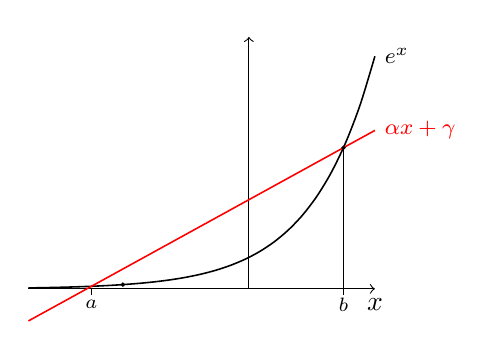
\begin{tikzpicture}[scale=0.8]
\draw[->] (-3.5,0) -- (2,0) node[anchor=north] {$x$};
\draw[->] (0,0) -- (0,4) node[anchor=east] {};
\draw[smooth, domain=-3.5:2.0, color=black, line width=0.20mm] 
    plot (\x,{e^(\x)/2}) node [right] {\footnotesize $e^x$};
\draw[smooth, domain=-3.5:2.0, color=red, line width=0.20mm] 
    plot (\x,{(   ((\x+2.5)*e^(1.5) + (1.5-\x)*e^(-2.5))/4    )/2}) node [right] {\footnotesize $\alpha x+\gamma$};
\draw (1.5,-0.1) -- (1.5,{e^(1.5)/2});
\draw (-2.5,-0.1) -- (-2.5,0);
\draw[black,fill] (1.5,{e^(1.5)/2}) circle (0.25mm);
\draw[black,fill] (-2,{e^(-2)/2}) circle (0.25mm);
\draw	(-2.5,-0.25) node{{\scriptsize $a$}}
		(1.5,-0.25) node{{\scriptsize $b$}};
\end{tikzpicture}

%\caption{A line over an exponential curve}%
\label{fig:graph1}
}
\end{figure}

\begin{theorem}[Hoeffding's inequality]\label{hoeffdings_inequality22}
Let $X$ be a real-valued random variable that is bounded $a\le X\le b$, with a mean $\mu$ of zero.  Then for $t>0$, the mean $\hat{\mu}$ of $n$ independent samples of $X$ is probability bounded by:
\begin{equation}\p(\hat{\mu}-\mu\ge t)\le \left( \frac{b}{b-a}\left(\frac{b(a-t)}{a(b-t)}\right)^{\frac{a-t}{b-a}} -\frac{a}{b-a}\left(\frac{b(a-t)}{a(b-t)}\right)^{\frac{b-t}{b-a}}  \right)^n
\end{equation}
\end{theorem}
\end{frame}

\begin{frame}
Or in an even more approximated form you might be familiar with: \cite{hoeffding1}
\begin{theorem}[Hoeffding's inequality]\label{Hoeffdings_inequality_proper}
Let $X$ be a real-valued random variable that is bounded $a\le X\le b$.  Then for $D=b-a$ and any $t>0$, the mean $\hat{\mu}$ of $n$ independent samples of $X$ is probability bounded by:
\begin{equation}\label{eq_no2}\p(\hat{\mu}-\mu\ge t)\le \exp\left(\frac{-2nt^2}{D^2}\right)
\end{equation}
\end{theorem}
%\begin{lemma}[Hoeffding's Lemma]\label{Hoeffdings_lemma_lemma}
%Let $X$ be a real-valued random variable that is bounded $a\le X\le b$, with a mean $\mu$ of zero, then for $D=b-a$ and any $s>0$:
%$$\E[\exp(sX)] \le \exp\left(\frac{1}{8}s^2D^2 \right)$$
%\end{lemma}
\end{frame}

\begin{frame}
Fitting a parabola becomes Bennett's inequality: \cite{hoeffding1,10.2307/2282438}

\begin{figure}[b]%
\centering
\parbox{2.0in}{

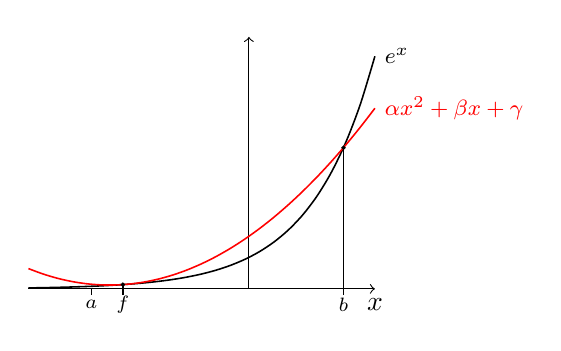
\begin{tikzpicture}[scale=0.8]
\draw[->] (-3.5,0) -- (2,0) node[anchor=north] {$x$};
\draw[->] (0,0) -- (0,4) node[anchor=east] {};
\draw[smooth, domain=-3.5:2.0, color=black, line width=0.20mm] 
    plot (\x,{e^(\x)/2}) node [right] {\footnotesize $e^x$};
\draw[smooth, domain=-3.5:2.0, color=red, line width=0.20mm] 
    plot (\x,{(0.316137167001903*\x*\x + 1.39988395124422*\x + 1.67055451771745)/2}) node [right] {\footnotesize $\alpha x^2+\beta x+\gamma$};
\draw (1.5,-0.1) -- (1.5,{e^(1.5)/2});
\draw (-2,-0.1) -- (-2,{e^(-2)/2});
\draw (-2.5,-0.1) -- (-2.5,0);
\draw[black,fill] (1.5,{e^(1.5)/2}) circle (0.25mm);
\draw[black,fill] (-2,{e^(-2)/2}) circle (0.25mm);
\draw	(-2.5,-0.25) node{{\scriptsize $a$}}
		(-2,-0.25) node{{\scriptsize $f$}}
		(1.5,-0.25) node{{\scriptsize $b$}};
\end{tikzpicture}

%\caption{A parabola over an exponential curve}%
\label{fig:graph1}}
\end{figure}

\begin{theorem}[Bennett's inequality]\label{hoeffdings1}
Let $X$ be a real-valued random variable with a mean of zero and variance $\sigma^2$, that is bounded $a\le X\le b$. 
Then for $t>0$, the mean $\hat{\mu}$ of $n$ samples of $X$ is probability bounded by:
\begin{equation}\label{eq_no2}\p(\hat{\mu}\ge t)\le \left(\left(\frac{\frac{\sigma^2}{b^2}}{\frac{\sigma^2}{b^2}+\frac{t}{b}}\right)^{\frac{\sigma^2}{b^2}+\frac{t}{b}}
\left(1-\frac{t}{b}\right)^{\frac{t}{b}-1}\right)^{\frac{n}{\frac{\sigma^2}{b^2}+1}}
\end{equation}
\end{theorem}
\end{frame}

%\begin{frame}
%Or simplify and turn into a handy-dandy lemma:
%\begin{lemma}\label{expectation1}
%For a random variable $X$ that is bounded on an interval $a\le X\le b$ with $D=b-a$ and variance $\sigma^2$, and any $s>0$:
%\[
%\E\left[\exp(s(X-\E[x]))\right] 
%\le\exp\left(\left(\frac{D^2}{17}+\frac{\sigma^2}{2}\right)s^2\right)
%\nonumber
%\]
%\end{lemma}
%\end{frame}

\begin{frame}
If we consider $X^2$ and then fit a parabola over a gaussian

\begin{figure}[b]%
\centering
\parbox{2.0in}{

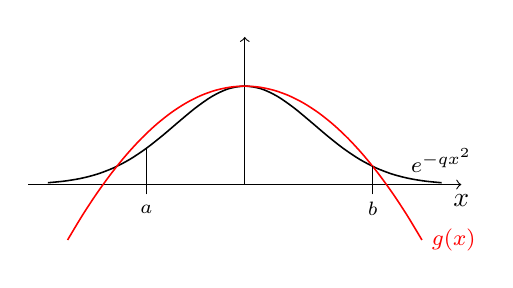
\begin{tikzpicture}[scale=1.25]
\draw[->] (-2.2,0) -- (2.2,0) node[anchor=north] {$x$};
\draw[->] (0,0) -- (0,1.5) node[anchor=east] {};
\draw[smooth, domain=-2.0:2.0, color=black, line width=0.20mm] 
    plot (\x,{e^(-(\x*\x))}) node [above] {\footnotesize $e^{-qx^2}$};
\draw[smooth, domain=-1.8:1.8, color=red, line width=0.20mm] 
    plot (\x,{-0.4825*\x*\x+1}) node [right] {\footnotesize $g(x)$};
\draw (1.3,-0.1) -- (1.3,{e^(-1.3*1.3)});
\draw (-1,-0.1) -- (-1,{e^(-1*1)});
\draw	(-1,-0.25) node{{\scriptsize $a$}}
		(1.3,-0.25) node{{\scriptsize $b$}};
\end{tikzpicture}

%\caption{A parabola over a gaussian curve}%
\label{fig:graph111}
}
\end{figure}

\begin{lemma}[Sample square bound]\label{sample_squares}
Let $X$ be a real-valued random variable with a mean of zero and variance $\sigma^2$, that is bounded $a\le X\le b$, if $d=\max(b,-a)$ then for $y>0$, the mean of sample squares $\hat{\sigma}_0^2=\frac{1}{n}\sum_ix_i^2$ is probability bounded:
\begin{equation}\label{equation_squares}\p(\sigma^2 - \hat{\sigma}_0^2> y) \le \left(
\left(\frac{1-\frac{\sigma^2}{d^2}}{1+\frac{y}{d^2}-\frac{\sigma^2}{d^2}}\right)^{1+\frac{y}{d^2}-\frac{\sigma^2}{d^2}}
\left(\frac{\frac{\sigma^2}{d^2}}{\frac{\sigma^2}{d^2}-\frac{y}{d^2}}\right)^{\frac{\sigma^2}{d^2}-\frac{y}{d^2}}
\right)^n
\end{equation}
\end{lemma}
\end{frame}

%\begin{frame}
%Equally turnable into a handy-dandy lemma
%\begin{lemma}\label{expectation2}
%Let $X$ be a random variable of finite support on an interval $a\le X\le b$, with $D=b-a$ and variance $\sigma^2 = \E[(X-\E[x])^2] = \E[X^2]-\E[X]^2$. Then for any $q>0$:
%$$\E[\exp(q(\sigma^2-(X-\E[X])^2))] \le \exp\left(\frac{1}{2}\sigma^2q^2D^2\right)$$
%\end{lemma}
%\end{frame}





\begin{frame}
\begin{figure}[h]
\centering
\begin{tikzpicture}[scale=0.9, transform shape,->,>=stealth',shorten >=1pt,auto,node distance=1.7cm,thick,main node/.style={circle}]
   % \path[use as bounding box] (-2.5cm, -2.8cm) rectangle (2.5cm, 2.5cm);
    \node[main node] (A1)  at (-5cm,-3cm) [align=center, text width=3.3cm] {\small Bound on Variable\\ in terms of its Width};
    \node[main node] (A2)  at (-5cm, 0cm) [align=center, text width=3.3cm] {\small Bound on Variable\\ in terms of its Variance\\ and Width};
    \node[main node] (A3)  at (-5cm, 3cm) [align=center, text width=3.3cm] {\small Bound on Variable Squared\\ in terms of its Width};
    \node[main node] (B1)  at (0cm, -3cm) [align=center, text width=3.3cm] {\small Bound on sum Square Errors};
    \node[main node] (B2)  at (0cm,  0cm) [align=center, text width=3.3cm] {\small Bound on Stratified mean\\ in terms of sum of \\strata variances};
    \node[main node] (B3)  at (0cm,  3cm) [align=center, text width=3.3cm] {\small Bound on Error of\\ sum of strata variances\\ in terms of sum square errors};
    \node[main node] (C1)  at (5cm,  0cm) [align=center, text width=3.3cm] {\small New Bound};


    \node[main node] (A1m)  at (-5cm,-3cm) [align=center, text width=3.2cm] {};
    \node[main node] (A2m)  at (-5cm, 0cm) [align=center, text width=3.2cm] {};
    \node[main node] (A3m)  at (-5cm, 3cm) [align=center, text width=3.2cm] {};
    \node[main node] (B1m)  at (0cm, -3cm) [align=center, text width=3.2cm] {};
    \node[main node] (B2m)  at (0cm,  0cm) [align=center, text width=3.2cm] {};
    \node[main node] (B3m)  at (0cm,  3cm) [align=center, text width=3.2cm] {};
    \node[main node] (C1m)  at (5cm,  0cm) [align=center, text width=3.2cm] {};

    \path[every node/.style={sloped,auto=false}]
(A1m) edge [line width=1pt,anchor=south] node {} (B1m)
(A2m) edge [line width=1pt,anchor=south] node {} (B2m)
(A3m) edge [line width=1pt,anchor=south] node {} (B3m) 

(B1m) edge [line width=1pt,anchor=south] node {} (C1)
(B2m) edge [line width=1pt,anchor=south] node {} (C1)
(B3m) edge [line width=1pt,anchor=south] node {} (C1) 
    ;
\end{tikzpicture}
\end{figure}
\end{frame}


\begin{frame}
\frametitle{Shapley Value sampling}

We test out how effective sampling to minimise this new bound is against other Shapley Value sampling methods:

\begin{enumerate}
\item	particularly simple sampling \cite{DBLP:journals/cor/CastroGT09}
\item	Neyman allocation \cite{CASTRO2017180,DBLP:journals/tsg/OBrienGR15}
\item	allocation to minimise Hoeffding's inequality \cite{2013arXiv1306.4265M}.
\end{enumerate}

\end{frame}




\begin{frame}
with ${\Omega}_m^n = {\Psi}_m^n = \frac{1}{m}$
\begin{equation}\label{big_equation}
%\p\left(\frac{\left|\sum_{i=1}^n\tau_i(\chi_{i,m_i}-\mu_i)\right|}{\sqrt{\log(6/p)}}\ge \sqrt{\begin{matrix*}[l]\sum_{i=1}^n\frac{4}{17}\Omega_{m_i}^{n_i}D_i^2\tau_i^2 \\ +\begin{pmatrix*}[l]\sqrt{\log(3/p)\left(\max_i\tau_i^2{\Psi_{m_i}^{n_i}}^2D_i^2\right)} \\ +\sqrt{\begin{matrix*}[l]2\sum_{i=1}^n\tau_i^2\Psi_{m_i}^{n_i}(m_i-1)\doublehat{\sigma}_i^2/m_i \\ + \log(6n/p)\sum_i\tau_i^2D_i^2\Omega_{m_i}^{n_i}\Psi_{m_i}^{n_i} \\ +\log(3/p)\left(\max_i\tau_i^2{\Psi_{m_i}^{n_i}}^2D_i^2\right)\end{matrix*}} \end{pmatrix*}^2\end{matrix*}}\right)
%\le p 
%\end{equation}
%\begin{equation}\label{big_equation_alternate}
\pr\left(\left|\sum_{i=1}^n\tau_i(\chi_{i,m_i}-\mu_i)\right| 
\ge \sqrt{\log(6/p)\left( \alpha
+ \left(\sqrt{\beta} 
+ \sqrt{\gamma}\right)^2\right) } \right)
\le p 
\end{equation}
where:
\begin{align*}
\alpha=&\sum_{i=1}^n\frac{4}{17}\Omega_{m_i}^{n_i}D_i^2\tau_i^2 \\
\beta=&\log(3/p)\left(\max_i\tau_i^2{\Psi_{m_i}^{n_i}}^2D_i^2\right) \\
\gamma=& 2\sum_{i=1}^n\tau_i^2\Psi_{m_i}^{n_i}(m_i-1)\doublehat{\sigma}_i^2/m_i
+ \log(6n/p)\sum_i\tau_i^2D_i^2\Omega_{m_i}^{n_i}\Psi_{m_i}^{n_i} \\
&\quad\quad\quad\quad\quad\quad\quad\quad\quad\quad\quad~+\log(3/p)\left(\max_i\tau_i^2{\Psi_{m_i}^{n_i}}^2D_i^2\right).
\end{align*}
\end{frame}


\begin{frame}





\begin{table*}[]
    \centering 
    \begin{minipage}[]{0.8\textwidth}
        \centering
        \caption{Airport Game Average Errors}\label{tab1}
			\begin{tabular}{llllll}
			\hline
			$\nicefrac{m}{n^2}$ & $10$ & $50$ & $100$ & $500$ & $1000$ \\
			\hline
			$e^{Ma}$   & 298.4 & 133.1 & 99.64 & 41.96 & 29.26 \\
			$e^{sim}$  & 357.8 & 146.1 & 106.2 & 44.55 & 36.33 \\
			$e^{Ca}$   & 325.7 & 115.8 & 75.85 & 31.01 & 22.12 \\
			$e^{SEBM}$ & 259.2 & 73.8 & 54.76 & 7.71 & 1.30  \\
			\hline
			\end{tabular}
    \end{minipage}
	\\\vspace{4mm}
    \begin{minipage}[]{0.8\textwidth}
        \centering
        \caption{Voting Game Average Errors}\label{tab2}
			\begin{tabular}{llllll}
			\hline
			$\nicefrac{m}{n^2}$ & $10$ & $50$ & $100$ & $500$ & $1000$ \\
			\hline
			$e^{Ma}$    & 131.0 & 57.78 & 41.52 & 18.66 & 13.18 \\
			$e^{sim}$   & 145.7 & 59.72 & 40.31 & 17.56 & 12.84 \\
			$e^{Ca}$    & 142.1 & 47.35 & 31.05 & 14.08 & 9.800 \\
			$e^{SEBM}$  & 122.8 & 47.44 & 33.18 & 8.55 & 1.995  \\
			\hline
			\end{tabular}
    \end{minipage}
	\\\vspace{4mm}
    \begin{minipage}[]{0.8\textwidth}
        \centering
        \caption{Simple Reward Division Game average errors}\label{tab3}
			\begin{tabular}{llllll}
			\hline
			$\nicefrac{m}{n^2}$ & $10$ & $50$ & $100$ & $500$ & $1000$ \\
			\hline
			$e^{Ma}$    & 25.68 & 11.62 & 7.792 & 3.481 & 2.290 \\
			$e^{sim}$   & 22.10 & 9.045 & 6.218 & 2.642 & 1.938 \\
			$e^{Ca}$    & 22.37 & 8.925 & 6.692 & 2.727 & 1.940 \\
			$e^{SEBM}$  & 19.25 & 7.044 & 5.158 & 1.183 & 0.2817  \\
			\hline
			\end{tabular}
    \end{minipage}
	\\\vspace{4mm}
    \begin{minipage}[]{0.8\textwidth}
        \centering
        \caption{Complex Reward Division Game average errors}\label{tab4}
			\centering
			\begin{tabular}{llllll}
			\hline
			$\nicefrac{m}{n^2}$ & $10$ & $50$ & $100$ & $500$ & $1000$ \\
			\hline
			$e^{Ma}$   & 276.1 & 118.9 & 87.00 & 40.15 & 27.44 \\
			$e^{sim}$  & 251.4 & 108.0 & 78.63 & 34.64 & 26.82 \\
			$e^{Ca}$   & 290.5 & 116.5 & 81.82 & 35.70 & 26.50 \\
			$e^{SEBM}$ & 214.2 & 78.47 & 54.10 & 12.45 & 2.711  \\
			\hline
			\end{tabular}
    \end{minipage}
    \vspace{3mm}
    \caption{Average absolute errors in the Shapley value calculation across all players in the four cooperative games (units in $10^{-4}$), for the different sampling schemes with different sampling budgets $m$ per number of strata (with $n^2=15^2$ for all).}
    \label{Table2}
\end{table*}

\end{frame}

\begin{frame}





\begin{table}[]
    \centering 
    \begin{minipage}[]{0.8\textwidth}
        \centering
        \caption{Simple Reward Division Game average errors}\label{tab3}
			\begin{tabular}{llllll}
			\hline
			$\nicefrac{m}{n^2}$ & $10$ & $50$ & $100$ & $500$ & $1000$ \\
			\hline
			$e^{Ma}$    & 25.68 & 11.62 & 7.792 & 3.481 & 2.290 \\
			$e^{sim}$   & 22.10 & 9.045 & 6.218 & 2.642 & 1.938 \\
			$e^{Ca}$    & 22.37 & 8.925 & 6.692 & 2.727 & 1.940 \\
			$e^{SEBM}$  & 19.25 & 7.044 & 5.158 & 1.183 & 0.2817  \\
			\hline
			\end{tabular}
    \end{minipage}
	\\\vspace{4mm}
    \begin{minipage}[]{0.8\textwidth}
        \centering
        \caption{Complex Reward Division Game average errors}\label{tab4}
			\centering
			\begin{tabular}{llllll}
			\hline
			$\nicefrac{m}{n^2}$ & $10$ & $50$ & $100$ & $500$ & $1000$ \\
			\hline
			$e^{Ma}$   & 276.1 & 118.9 & 87.00 & 40.15 & 27.44 \\
			$e^{sim}$  & 251.4 & 108.0 & 78.63 & 34.64 & 26.82 \\
			$e^{Ca}$   & 290.5 & 116.5 & 81.82 & 35.70 & 26.50 \\
			$e^{SEBM}$ & 214.2 & 78.47 & 54.10 & 12.45 & 2.711  \\
			\hline
			\end{tabular}
    \end{minipage}
    \vspace{3mm}
    \caption[Average errors approximating the Shapley Value across games and methods]{Average absolute errors in the Shapley value calculation across all players in the four cooperative games (units in $10^{-4}$), for the different sampling schemes with different sampling budgets $m$ per number of strata (with $n^2=15^2$ for all).}
    \label{Table2}
\end{table}

\end{frame}

